%%%%%%%%%%%%%%%%%%%%%%%%%%%%%%%%%%%%%%%%%%%%%%
%                insertmeeting
% 1) Title (something creative & funny?)
% 2) Date (MM/DD/YYYY)
% 3) Location (ex. Hagerty High School)
% 4) People/Committees Present 
% 5) Picture 
% 6) Start Time & Stop Time (ex. 12:30AM to 4:30PM)
%%%%%%%%%%%%%%%%%%%%%%%%%%%%%%%%%%%%%%%%%%%%%%
\insertmeeting 
	{We Are Going On Forbes} 
	{04/18/22} 
	{Hagerty High School}
	{Annika, Anouska, Clayton, Falon, James, Jensen, Nathan, Ritam, Rose, Samantha, Lilly}
	{Images/RobotPics/robot.jpg}
	{2:30 - 4:30}
	
\hhscommittee{Outreach}
\noindent\hfil\rule{\textwidth}{.4pt}\hfil
\subsubsection*{Goals}
\begin{itemize}
    \item Forbes Interview with Janet Burns


\end{itemize} 

\noindent\hfil\rule{\textwidth}{.4pt}\hfil

\subsubsection*{Accomplishments}
After a 5 year long break, we reached out to Forbes magazine to interview for a report about the up and coming world competition. Ms. Janet Burns, a senior contributer and freelance writer on consumer technology, questioned our team and listened to our world's presentation script. We were able to discuss the multi faceted nature of FIRST and elaborated on the new technology we are using within our robot as well as our outreach program. She was shocked to see how much our team has developed in 5 years and the advancement of the techonology we are using. Among other things we focused on the customized parts on the robot as well as our teams collaboration and FIRST's embodiment of Gracious Professionalism. 

\begin{figure}[htp]
\centering
\includegraphics[width=0.95\textwidth, angle=0]{Meetings/April/04-18-22/04-18-22 1.JPG}
\caption{The team in action}
\label{fig:041822_1}
\end{figure}

\begin{figure}[htp]
\centering
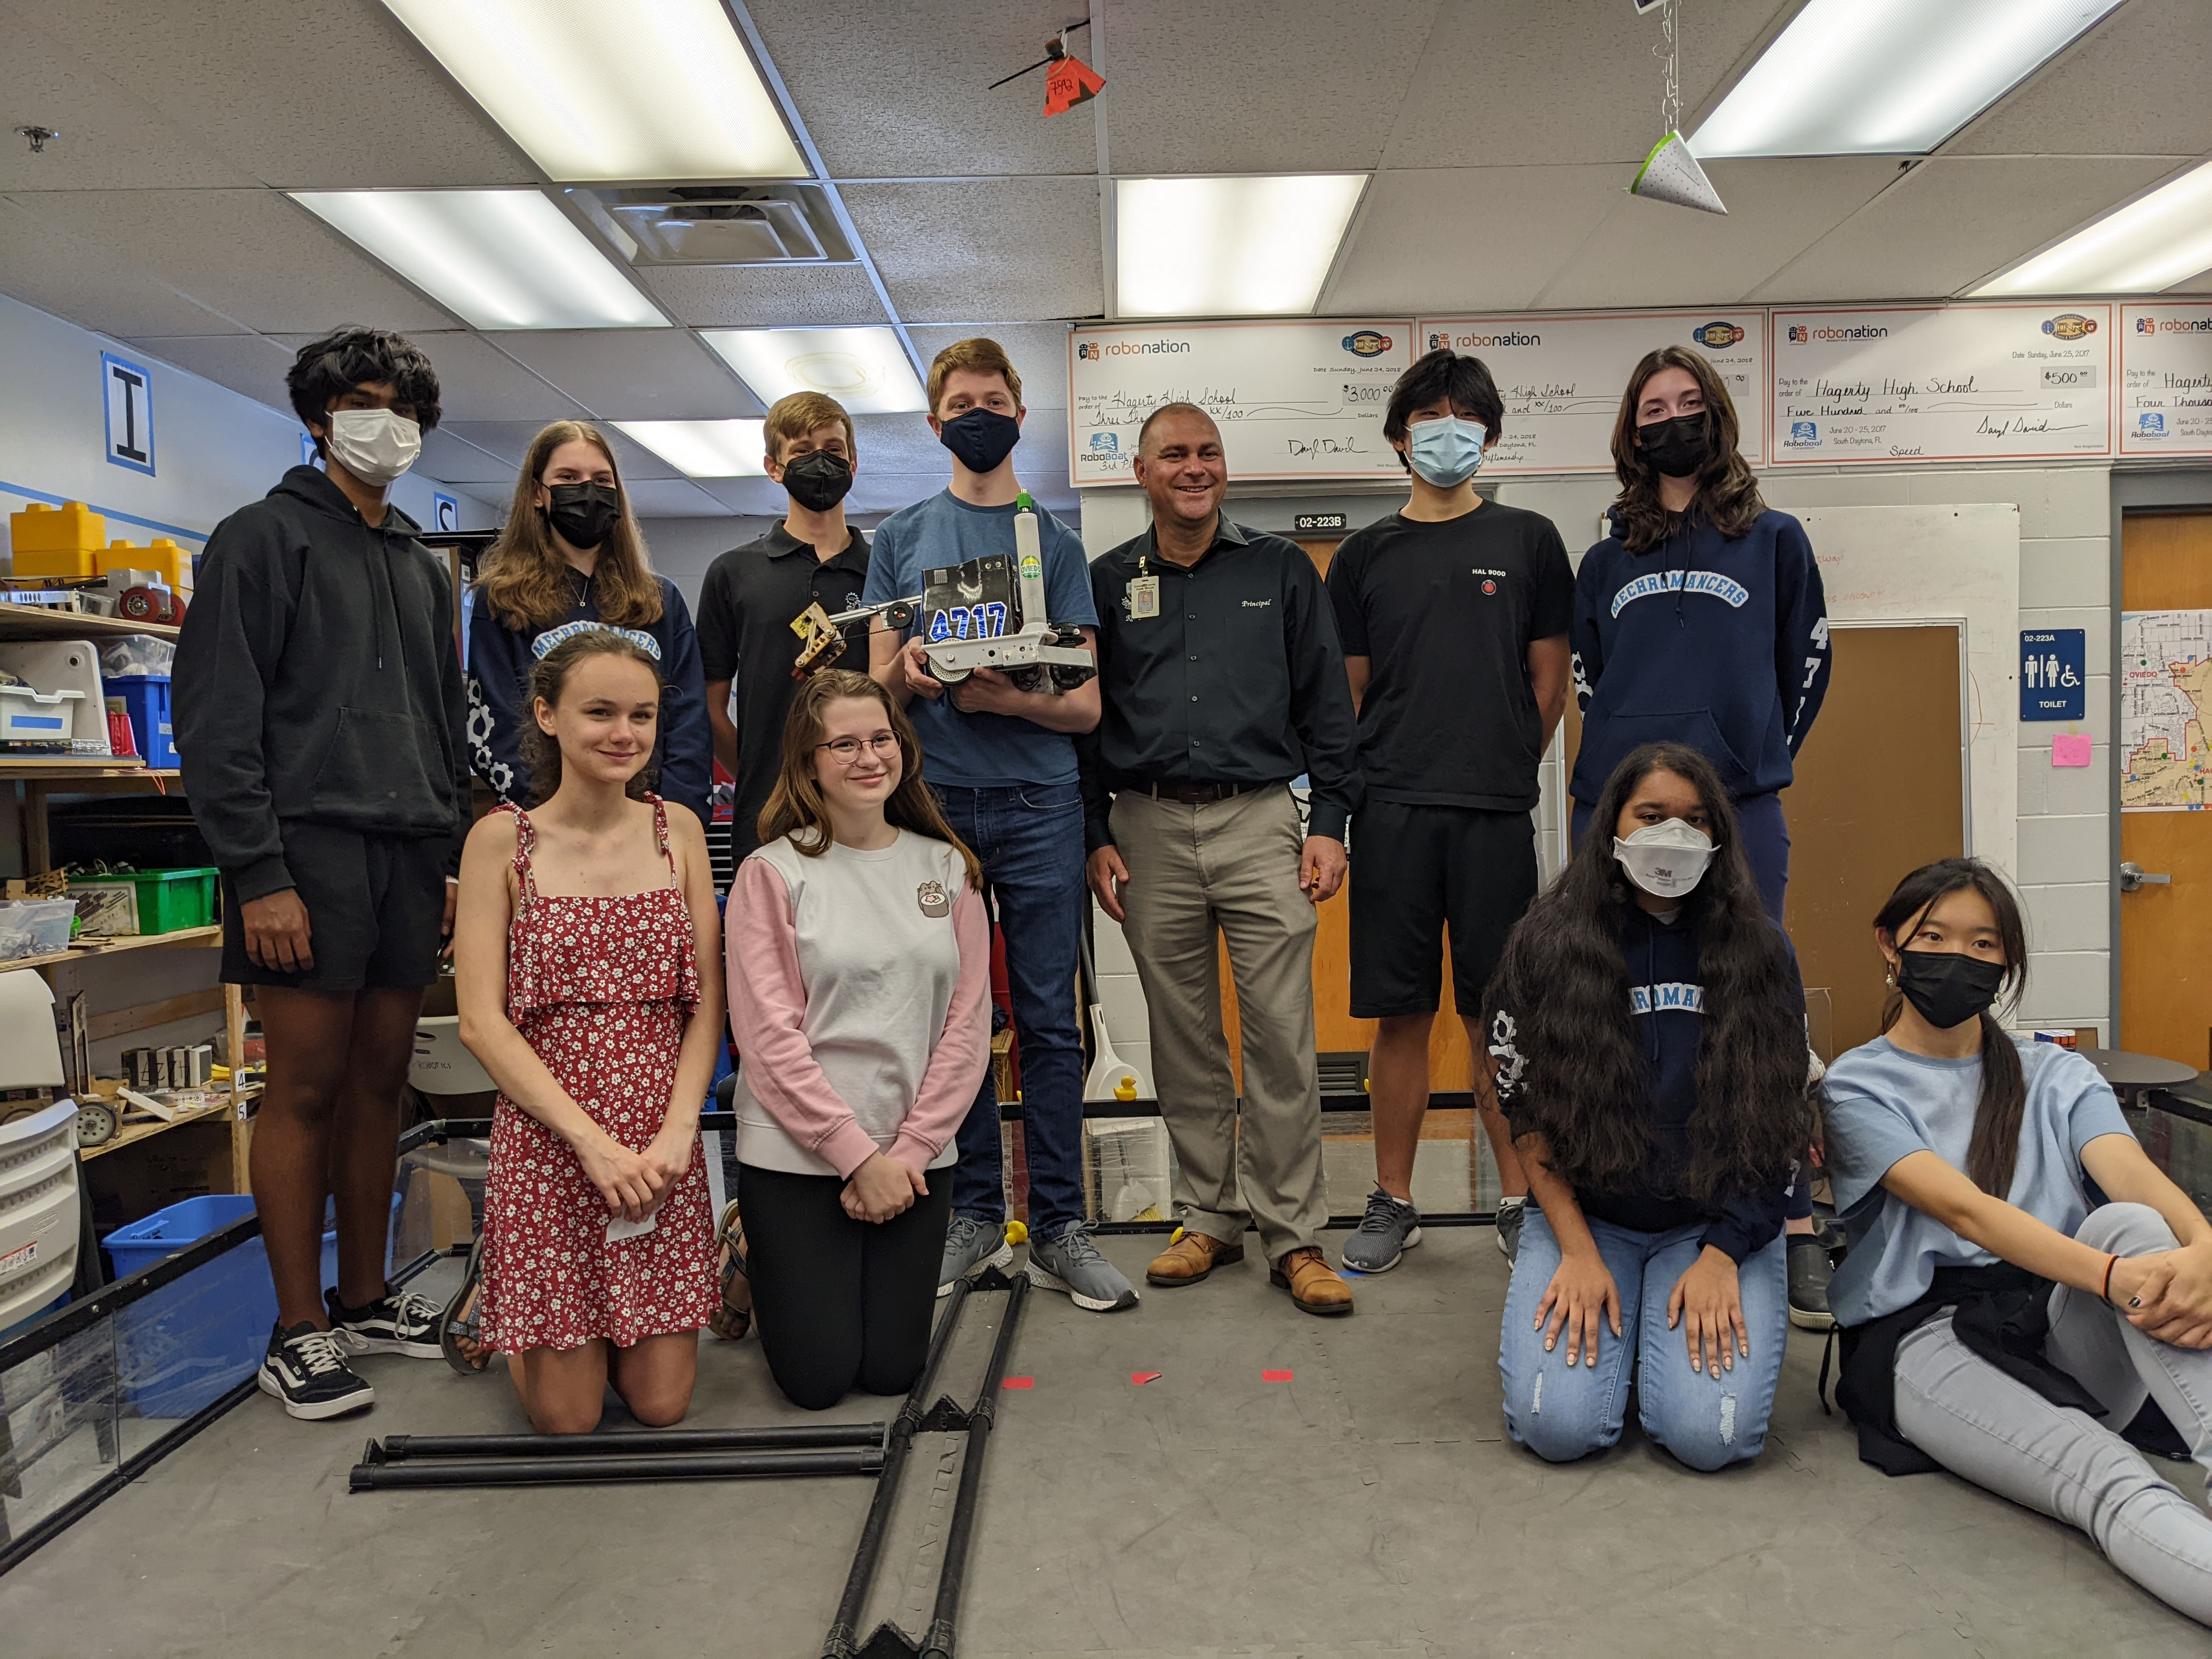
\includegraphics[width=0.95\textwidth, angle=0]{Meetings/April/04-18-22/04-18-22 2.JPG}
\caption{Picture with Mr. Frasca, Hagerty High School's Principal}
\label{fig:041822_2}
\end{figure}



\whatsnext{
\begin{itemize}
    \item Reach out to local news firms 
\end{itemize} 
}

